\documentclass[11pt]{article}
\usepackage{amsmath,amssymb,amsthm}
\usepackage{graphicx}
\usepackage[colorlinks=true,linkcolor=blue,citecolor=blue]{hyperref}

\newtheorem{theorem}{Theorem}[section]
\newtheorem{lemma}[theorem]{Lemma}
\newtheorem{proposition}[theorem]{Proposition}
\newtheorem{corollary}[theorem]{Corollary}
\theoremstyle{definition}
\newtheorem{definition}[theorem]{Definition}

\newcommand{\tr}{\operatorname{Tr}}
\newcommand{\supp}{\operatorname{supp}}
\DeclareMathOperator{\Enc}{Enc} \DeclareMathOperator{\Dec}{Dec}
\DeclareMathOperator{\Eval}{Eval} \DeclareMathOperator{\KeyGen}{KeyGen}

\title{\bfseries UP-QFHE: Uncloneable Quantum Fully Homomorphic Encryption\\
of Classical Data via a Single Pad Register}
\author{David S.~(dspaid)}
\date{November 2026 --- code and experiments at \url{https://github.com/dspaid/dail-bnty-0736}}

\begin{document}
\maketitle

\begin{abstract}
We give a one-time, private-key quantum fully homomorphic encryption scheme for
classical messages and classical circuits over $\{\mathsf{NOT},\mathsf{AND}\}$
in which the secret of a classical one-time pad is stored in an \emph{uncloneable
quantum register}: $n$ BB84 qubits prepared with a random basis key $\theta$.
Because the encrypted payload is always a computational-basis state, homomorphic
evaluation is \emph{exact at any depth} --- no noise, no bootstrapping, no
lattice assumption --- and the evaluator's entire view (the padded transcript)
is shown to be identically distributed for every message, i.e.\ input
confidentiality is information-theoretic.  What cannot be duplicated is the pad
register: we analyse the key-revealing splitting game in which one ciphertext is
split between two isolated parties who are both then shown $\theta$ and must
decrypt.  The one-bit game value is \emph{exactly $3/4$} over all quantum
attacks; the proof is a complete dual-certificate argument carried out in this
paper ($Y=\tfrac38 I_2$ feasible, gap matrix positive semidefinite with an
exact rational spectrum) matched by an explicit optimal Kraus pair, and
tensoring gives $p_n^\ast = (3/4)^n$ for joint attacks on $n$ bits.  Every claim is backed by
runnable code in the accompanying repository: the full test suite, two seeded
experiment scripts, and the resulting JSON logs reproduce every number quoted
here on a clean machine with no API keys.
\end{abstract}

\section{Introduction}

Uncloneable encryption --- encrypting so that a single ciphertext cannot be
copied into two halves that both decrypt correctly after the key is revealed
--- has a long lineage from Wiesner's conjugate coding through the formal game
of Broadbent and Lord~\cite{bl20}, who showed that uncloneable encryption needs
oracles for general messages.  A wave of recent work removed the assumptions:
Ananth and Sahai~\cite{as26} gave an unconditional one-bit scheme, Bhattacharyya,
Broadbent and Culf~\cite{bbc26} upgraded it to statistically secure encryption
of arbitrary messages, and Broadbent, Culf and Rochette~\cite{bcr26} mapped the
landscape of untelegraphable encryption with optimal bounds.  On a parallel
track, Broadbent and Jeffery~\cite{bj15} defined quantum homomorphic encryption
of \emph{classical} circuits (QFHE): quantum ciphertexts carrying classical
data that a quantum evaluator processes without learning the data.

This paper fuses the two lines at their simplest points and works the
quantitative details out completely.  The object is a one-time private-key
QFHE scheme whose one-time-pad secret lives in an uncloneable register:
\emph{the thing the homomorphic evaluator must not be able to duplicate is
exactly the pad}.  Two properties are proved and verified by code:

\begin{itemize}
\item \textbf{Exact unbounded-depth evaluation.}  The payload register is always
a $\{|0\rangle,|1\rangle\}$-basis state, so a circuit over
$\{\mathsf{NOT},\mathsf{AND}\}$ can be evaluated by physically driving the
payload qubits and, equivalently, by simulating the \emph{padded transcript}
$C(x \oplus a)$ classically (Definition~\ref{def:eval}).  Theorem~\ref{thm:secret}
shows the transcript distribution is identical for all messages $x$: perfect
input confidentiality, one time, unconditionally.  (Correspondingly, the scheme
is not \emph{compact}: the transcript is the price of exact non-linear
evaluation without an oracle.)
\item \textbf{Quantified uncloneability.}  In the key-revealing splitting game
(Definition~\ref{def:game}) the adversary holds one ciphertext, splits it by any
quantum operation, and two isolated parties --- each shown $\theta$ --- must both
recover the message.  Theorem~\ref{thm:value} proves the one-bit value is
exactly $3/4$: the explicit dual certificate $Y = \tfrac38 I_2$
(Appendix~\ref{app:cert}) bounds every attack from above, and an explicit
trace-preserving Kraus pair, displayed in the proof, attains it.
Corollary~\ref{cor:nbit} upgrades this to $p_n^\ast = (3/4)^n$ for arbitrary
joint attacks on $n$ ciphertext qubits.  Naive strategies get only $(5/8)^n$.
\end{itemize}

The scope is deliberately narrow (Section~\ref{sec:scope}): classical messages,
one-time use, private key, $\{\mathsf{NOT},\mathsf{AND}\}$ circuits, and security
against a splitting adversary with honest decoders.  Within that scope every
statement is fully proved and every constant is computed by the repository's
code rather than quoted from elsewhere.

\paragraph{Related work.}
Conjugate-coding uncloneability goes back to Wiesner; Bennett--Wiesner~\cite{bw84}
is the published ancestor of the BB84 states used here.  The splitting-game
formalism is that of Broadbent--Lord~\cite{bl20} (their oracle lower/upper bounds
are for general messages; our contribution is not a competitor to their or to
the recent unconditional schemes~\cite{as26,bbc26,bcr26}, which encrypt quantum
messages, whereas here the message is classical and the uncloneable register
plays the role of the pad).  The QFHE-for-classical-circuits setting and its
blind-evaluation structure are from Broadbent--Jeffery~\cite{bj15}.  The dual
certificate method for bounding two-player quantum games is standard
(Choi--Jamio{\l}kowski representation and semidefinite-program weak duality;
see Watrous~\cite{watrous} for the channel formalism).

\section{Preliminaries}\label{sec:prelim}

All qubit registers are listed with qubit~0 as the most significant tensor
factor in statevector conventions of the code (\texttt{qfhe/sim.py}).  For
$\theta \in \{0,1\}$ and $b \in \{0,1\}$ write
\[
  |u_b^\theta\rangle \;=\; H^{\theta}|b\rangle, \qquad
  |u_0^0\rangle=|0\rangle,\ |u_1^0\rangle=|1\rangle,\
  |u_0^1\rangle=|+\rangle,\ |u_1^1\rangle=|-\rangle ,
\]
and for strings $u = u_1 \oplus a$ denotes bitwise XOR.  A boolean circuit $C$
is a gate list over $\{\mathsf{NOT},\mathsf{AND}\}$ acting on $n$ wires;
$\mathsf{AND}$ is applied as $w_t \mathrel{|}= w_a \wedge w_b$ with the target
wire distinct from both controls (the code raises otherwise, since XOR-accumulated
$\mathsf{AND}$ with $t \in \{a,b\}$ is classically irreversible).  A channel
$\Lambda: \mathcal{L}(\mathbb{C}^2) \to \mathcal{L}(\mathbb{C}^4)$ has Choi
matrix $J_\Lambda = \sum_{i,j} |i\rangle\langle j| \otimes \Lambda(|i\rangle\langle j|)$,
so that $\Lambda$ is completely positive iff $J_\Lambda \succeq 0$ and
trace-preserving iff $\tr_{AB} J_\Lambda = I_2$~\cite{watrous}.

\section{The scheme}\label{sec:scheme}

\begin{definition}[uncloneable pad]\label{def:pad}
For a basis key $\theta \in \{0,1\}^n$ and value $a \in \{0,1\}^n$ the pad
register is
$\mathrm{Pad}_\theta(a) = \bigotimes_{j=1}^{n} |u_{a_j}^{\theta_j}\rangle$.
More generally the key may be a random Clifford circuit $V$ on $n$ qubits with
$\mathrm{Pad}_V(a) = V|a\rangle$ (\texttt{qfhe/pad.py}, functions
\texttt{bb84\_encode} and \texttt{clifford}); both are key-randomised Cliffords
applied to a $Z$-basis string.
\end{definition}

\begin{definition}[UP-QFHE]\label{def:scheme}
$\KeyGen(1^n)$: sample $\theta \leftarrow \{0,1\}^n$ uniformly; key $k=\theta$.

$\Enc_k(x)$ for $x \in \{0,1\}^n$: sample pad $a \leftarrow \{0,1\}^n$ uniform;
prepare the \emph{payload} register in $|x \oplus a\rangle$ ($Z$ basis) and the
\emph{mask} register in $\mathrm{Pad}_\theta(a)$.  Ciphertext
$\mathsf{ct} = (\mathsf{pay}, \mathsf{mask})$.

$\Dec_k(\mathsf{ct})$: measure mask qubit $j$ in basis $\theta_j$ to recover
$a_j$ (exact: the key holder knows the encoding basis); output $x = p \oplus a$
where $p$ is the read-out of the payload register.
\end{definition}

Correctness is immediate: $|x\oplus a\rangle$ and $\Dec$'s exact recovery of $a$
give $x$ with probability~1 (\texttt{tests/test\_scheme.py}).

\begin{definition}[homomorphic evaluation]\label{def:eval}
Given a circuit $C$ over $\{\mathsf{NOT},\mathsf{AND}\}$ the evaluator, without
touching the mask register, (i) applies the circuit physically to the payload
qubits --- $\mathsf{NOT} \mapsto X$, $\mathsf{AND} \mapsto \mathsf{CCX}$
($\mathsf{CX}$ when both controls coincide), and (ii) produces the classical
transcript $p_{\mathrm{out}} = C(p_{\mathrm{in}})$, where
$p_{\mathrm{in}}$ is any read-out of the payload register before evaluation.
The key holder computes $C(x) = C(p_{\mathrm{in}} \oplus a)$ from
$p_{\mathrm{in}}$ and $\Dec_k$.
\end{definition}

Because the payload stays a $Z$-basis state at every step, the physical pass and
the transcript agree exactly, and neither is limited by depth: this is exact
unbounded-depth homomorphic evaluation.  The transcript is what Definition~\ref{def:eval}
releases to make non-linear gates work without an oracle; for $\mathsf{NOT}$-only
circuits even that release is unnecessary (Lemma~\ref{lem:not}).

\begin{theorem}[uncloneability of the ciphertext]\label{thm:secret}
Fix $n$ and any message $x$.  In the key-revealing splitting experiment of
Definition~\ref{def:game} applied to $\Enc_k(x)$ with honest decoders, two
isolated parties both output the full message $C(x)$ with probability at most
$(3/4)^n$, for every joint quantum attack on the ciphertext.
\end{theorem}

\begin{proof}
The payload register is a $Z$-basis state, so the adversary may copy and
distribute it perfectly; no strategy can do better than that, and the payload
carries no uncloneable content.  Each decoder's guess of $x$ (hence of $C(x)$)
is a function of its own mask half and $\theta$; both decoders succeed at the
full string iff both recover all $n$ pad bits correctly, which is exactly the
$n$-bit key-revealing game on $\mathrm{Pad}_\theta(a)$ bounded by
$(3/4)^n$ in Corollary~\ref{cor:nbit}.
\end{proof}

\begin{theorem}[perfect input confidentiality of the transcript]\label{thm:sec2}
For every circuit $C$, the evaluator's complete view
$(p_{\mathrm{in}}, p_{\mathrm{out}}) = (u, C(u))$ with $u$ uniform on
$\{0,1\}^n$, is identically distributed for all messages $x$.  In particular no
computationally unbounded adversary learns anything about $x$ from the view;
and the payload register alone, averaged over $a$, is maximally mixed.
\end{theorem}

\begin{proof}
$a$ is uniform and independent of $x$, so $p_{\mathrm{in}} = x \oplus a$ is
uniform and independent of $x$, and $p_{\mathrm{out}}$ is a deterministic
function of $p_{\mathrm{in}}$.  Hence the view is $(u, C(u))$ for uniform $u$,
regardless of $x$.  The payload ensemble $\{ |x \oplus a\rangle : a
\leftarrow \{0,1\}^n\}$ is the uniform mixture over all $2^n$ basis states.
\end{proof}

\begin{lemma}[blind frame flip]\label{lem:not}
Applying $X$ to payload qubit $j$ flips the encrypted bit $x_j$ whatever the
key $\theta$ and pad $a$ are: $p_j \mapsto p_j \oplus 1$ and
$\Dec_k$ outputs $x \oplus e_j$.  Thus $\mathsf{NOT}$ gates need no access to
the mask register at all, quantumly or classically.
\end{lemma}

\begin{proof}
The payload is a $Z$-basis state independent of the mask; $X$ complements its
bit, and XOR decryption is equivariant under that complement.  Verified as a
physical circuit identity over random keys in\\
\texttt{tests/test\_scheme.py::test\_x\_frame\_flips\_pad\_bit\_blindly}.
\end{proof}

\section{The key-revealing splitting game}\label{sec:game}

\begin{definition}[one-bit game $G_1$]\label{def:game}
A bit is encoded as $|u\rangle \in \{|0\rangle,|1\rangle,|+\rangle,|-\rangle\}$
with each state chosen with probability $1/4$; the basis key $\theta$ is
\emph{not} revealed to the adversary, who holds one copy and applies any CPTP
map $\Lambda: \mathbb{C}^2 \to \mathbb{C}^2 \otimes \mathbb{C}^2$ producing
systems $A$ and $B$.  The two decoders are then each shown $\theta$ and measure
their system in the $\theta$ basis (honest decryption); the adversaries win iff
\emph{both} outputs equal the encoded bit.  Let $p_1^\ast$ be the supremum over
all attacks, and $p_n^\ast$ the analogous value for $n$ independent pads with
arbitrary joint attacks and both decoders required to get all $n$ bits.
\end{definition}

For real states $u$ the winning probability of an attack $\Lambda$ is
\begin{equation}\label{eq:objective}
  p(\Lambda) \;=\; \frac14 \sum_{u} \langle uu|\, \Lambda(|u\rangle\langle u|)\, |uu\rangle
  \;=\; \tr\!\big[M\, J_\Lambda\big], \qquad
  M = \frac14 \sum_u |u\rangle\langle u| \otimes |uu\rangle\langle uu| ,
\end{equation}
the sum over the four BB84 states.  Every CPTP map is a physically realisable
split (Stinespring with an ancilla discarded inside the decoder's lab), so
$p_1^\ast = \max\{\tr[MJ] : J \succeq 0,\ \tr_{AB} J = I_2\}$.

\begin{proposition}[naive attacks]\label{prop:naive}
Copy-in-$Z$ (isometry $|b\rangle \mapsto |bb\rangle$) and copy-in-$X$ each win
with probability $5/8$; discarding and emitting a fixed state wins $3/8$.  For
copy-in-$Z$ the per-state probabilities are $(1, 1, \tfrac12, 0)$ on
$(|0\rangle, |1\rangle, |+\rangle, |-\rangle)$: the two halves of $|+\rangle$
are perfectly correlated in the $X$ basis but only half the time equal to $|+\rangle$,
and $|-\rangle$ is anti-correlated and always loses.
\end{proposition}

\begin{proof}
Direct evaluation of \eqref{eq:objective}; computed as
\texttt{p\_win\_isometry} in \texttt{qfhe/games.py} and asserted to $10^{-12}$
in \texttt{tests/test\_games.py}.
\end{proof}

\begin{proposition}[coherent isometries are still not optimal]\label{prop:iso}
Optimising \eqref{eq:objective} over splitting \emph{isometries}
$\mathbb{C}^2 \to \mathbb{C}^4$ by multi-start numerical search finds value
$\ge 0.72855$, strictly between $5/8$ and $3/4$; general channels do strictly
better (Theorem~\ref{thm:value}), so the isometry-restricted value is a lower
bound only.
\end{proposition}

\begin{theorem}[the game value is exactly $3/4$]\label{thm:value}
$p_1^\ast = 3/4$.  The maximum is attained by the explicit channel
$\Lambda^\ast(\rho) = A_1 \rho A_1^\dagger + A_2 \rho A_2^\dagger$ displayed in
the proof; it is not attained by any isometric split, nor by
measure-$Z$-and-reprepare, which only reaches $5/8$.
\end{theorem}

\begin{proof}
\textbf{Upper bound.}  Let $Y = \tfrac38 I_2$ and let $M$ be as in
\eqref{eq:objective}.  Appendix~\ref{app:cert} proves the gap matrix
$S := Y \otimes I_4 - M$ is positive semidefinite, using only exact rational
arithmetic: $16M$ is an explicit integer matrix and $\chi_M(\lambda) =
\lambda^4 (\lambda - \tfrac18)^2 (\lambda - \tfrac38)^2$, so every eigenvalue of
$M$ is at most $\tfrac38$.  For any channel $\Lambda$ with Choi matrix $J$:
\[
  p(\Lambda) = \tr[MJ] \;\le\; \tr\big[(Y \otimes I_4)\, J\big]
  \;=\; \tr\big[Y \underbrace{\tr_{AB} J}_{= I_2}\big] \;=\; \tr Y \;=\; \tfrac34 ,
\]
where the inequality is $J \succeq 0$ and $S \succeq 0$.  This is SDP weak
duality with an explicit dual-feasible point.

\textbf{Lower bound: an explicit optimal channel.}  Set $s := 1/\sqrt{12}$ and,
in the computational basis (input $\to$ output $\lvert a\rangle_A\lvert b\rangle_B$,
index $2a + b$),
\[
A_1 \;=\; s \begin{pmatrix} 3&0\\ 0&1\\ 0&1\\ 1&0\end{pmatrix},
\qquad
A_2 \;=\; (X \otimes X)\, A_1\, X \;=\; s \begin{pmatrix} 0&1\\ 1&0\\ 1&0\\ 0&3
\end{pmatrix}.
\]
Equivalently $A_1\lvert 0\rangle = (3\lvert 00\rangle + \lvert 11\rangle)/
\sqrt{12}$, $A_1\lvert 1\rangle = (\lvert 01\rangle + \lvert 10\rangle)/
\sqrt{12}$, and $A_2$ is $A_1$ with the input bit and both output bits flipped.  Trace preservation is direct:
$A_1^\dagger A_1 = \operatorname{diag}(\tfrac56, \tfrac16)$ and $A_2^\dagger
A_2 = \operatorname{diag}(\tfrac16, \tfrac56)$, whose sum is $I_2$.  (Neither is
a scalar multiple of $I$, so $\Lambda^\ast$ is a genuine channel, not an
isometry.)  Winning probabilities: the amplitude of $\Lambda^\ast$'s Kraus
images on $\lvert uu\rangle$ gives
\[
P_{\mathrm{win}}(0) = \Big|\tfrac{3}{\sqrt{12}}\Big|^2 = \tfrac34, \qquad
P_{\mathrm{win}}(1) = \Big|\tfrac{3}{\sqrt{12}}\Big|^2 = \tfrac34 \ \text{via } A_2,
\]
and for $\lvert\pm\rangle$, both branches contribute amplitude
$\pm 3/\sqrt{24}$ on $\lvert \pm,\pm\rangle$, so $P_{\mathrm{win}}(\pm) =
\tfrac{9}{24} + \tfrac{9}{24} = \tfrac34$.  Hence $p_1(\Lambda^\ast) = \tfrac34$,
and with the upper bound, $p_1^\ast = \tfrac34$ exactly.  In SDP language this
is complementary slackness: $\operatorname{vec}(A_1), \operatorname{vec}(A_2)$
are exactly the two basis vectors spanning $\ker\big(\tfrac38 I_{16} - M\big)$
(Appendix~\ref{app:cert}).

\textbf{Numerics.}  A multi-start Kraus search (rank~2, which suffices for
qubit $\to$ two-qubit channels) converges to value $0.75 + O(10^{-13})$, the
$\pm10^{-13}$ slack being the trace-preservation tolerance of the constrained
optimiser (\texttt{channel\_splitting\_value}, \texttt{results/games.json});
its fixed points have entries in
$\{0, \pm 1, \pm 3\}/\sqrt{12}$, i.e.\ the search rediscovers $\Lambda^\ast$,
which \texttt{optimal\_channel} implements exactly and
\texttt{tests/test\_games.py} re-verifies to machine precision (trace
preservation, value $3/4$ on each of the four states, and
$\operatorname{vec}(A_k) \in \ker(\tfrac38 I - M)$).
The optimum is not reached by any isometric split: equality in the upper
bound forces $\operatorname{vec}(V)$ into the $3/8$-eigenspace of $M$, spanned
by $(3|000\rangle + |011\rangle + |101\rangle + |110\rangle)/\sqrt{12}$ and
$(|001\rangle + |010\rangle + |100\rangle + 3|111\rangle)/\sqrt{12}$: an
$\alpha\beta$-combination is of the form $\operatorname{vec}(V)$ only if
$\langle V0 | V1\rangle = \alpha\bar\beta/6 = 0$, and $\alpha = 0$ or
$\beta = 0$ breaks normalisation of $V|0\rangle$ or $V|1\rangle$.  So no
isometry attains $3/4$ (the best found numerically is $0.72855\ldots$,
Proposition~\ref{prop:iso}), and measure-$Z$-and-reprepare achieves only
$\tfrac14(1 + 1 + \tfrac14 + \tfrac14) = 5/8$.
\end{proof}

\begin{corollary}[$n$ pads]\label{cor:nbit}
$p_n^\ast = (3/4)^n$: no joint attack on the $n$-qubit pad register
(including entangling splits and collective measurements) does better, and the
bound is attained by tensoring the optimal one-bit channel.
\end{corollary}

\begin{proof}
The $n$-bit objective operator is $M_n = M^{\otimes n}$ (winning all bits is the
product of winning each coordinate game), and $S_1 \succeq 0$ tensors to
$S_n = Y^{\otimes n} \otimes I_{4^n} - M_n \succeq 0$.  For any channel
$\Lambda_n$ with Choi matrix $J_n$:
$p_n(\Lambda_n) \le \tr[(Y^{\otimes n} \otimes I) J_n] = \tr[Y^{\otimes n}] = (3/4)^n$,
using $\tr_{AB} J_n = I_{2^n}$.  Conversely, the channel $\Lambda^\ast$ of
Theorem~\ref{thm:value} attains $3/4$ exactly; its $n$-fold tensor product is
trace-preserving and wins each coordinate independently with probability
$3/4$, so the upper bound is attained: $p_n^\ast = (3/4)^n$.  The empirical
scheme-specific attack below (naive per-qubit $Z$ copy) sits at $(5/8)^n$.
\end{proof}

\subsection{Numbers computed by the repository}

All values in this subsection are produced by \texttt{scripts/run\_games.py}
(fixed seeds) into \texttt{results/games.json}, and re-checked by
\texttt{tests/test\_games.py}.  Table~\ref{tab:onebit} lists the one-bit game;
Figure~\ref{fig:nbit} and Table~\ref{tab:nbit} show the end-to-end $n$-bit
scheme game, in which the ciphertext of Definition~\ref{def:scheme} is split by
the naive $Z$-copy isometry on each pad qubit (implemented by
\texttt{scheme\_splitting\_game}, whose per-bit bound is therefore $(5/8)^n$).

\begin{table}[h]
\centering
\begin{tabular}{lrl}
\hline
attack & value & method \\
\hline
copy in $Z$ / copy in $X$ (isometries) & $0.625 = 5/8$ & exact formula \\
discard, emit fixed state & $0.375 = 3/8$ & exact formula \\
best isometry found (40 restarts) & $0.72855\ldots$ & numerics, lower bound \\
explicit channel $\Lambda^\ast$, $p_1(\Lambda^\ast)$ & $0.75$ exact & analytic, Thm.~\ref{thm:value} \\
best CPTP channel found (Kraus rank 2) & $0.75000000000024$ & numerics \\
dual certificate $Y = \tfrac38 I_2$, $\tr Y$ & $0.75$ exact & analytic, App.~\ref{app:cert} \\
dual search certified bound & $0.75 + 4.1\times 10^{-9}$ & numerics \\
\hline
\end{tabular}
\caption{One-bit game $G_1$.  The gap matrix spectrum $\{0,0,\tfrac14,\tfrac14,
\tfrac38,\tfrac38,\tfrac38,\tfrac38\}$ (Appendix~\ref{app:cert}) certifies the
upper bound; the two-dimensional zero eigenspace of the gap is exactly
$\operatorname{span}\{\operatorname{vec}(A_1), \operatorname{vec}(A_2)\}$, the
Kraus pair of $\Lambda^\ast$ (complementary slackness).}
\label{tab:onebit}
\end{table}

\begin{table}[h]
\centering
\begin{tabular}{rrrrr}
\hline
$n$ & trials & $p_{\text{both}}$ & $p_{\ge 1}$ & bound $(5/8)^n$ \\
\hline
3 & 4000 & 0.2545 & 0.6045 & 0.2441 \\
4 & 4000 & 0.15625 & 0.4815 & 0.1526 \\
5 & 4000 & 0.104 & 0.3975 & 0.0954 \\
\hline
\end{tabular}
\caption{$n$-bit scheme game with the naive per-qubit $Z$-copy attack;
$p_{\text{both}}$ agrees with $(5/8)^n$ within statistical noise ($\pm 0.006$
at $1\sigma$, 4000 trials), and both are far below the information-theoretic
ceiling $(3/4)^n$.}
\label{tab:nbit}
\end{table}

\begin{figure}[h]
\centering
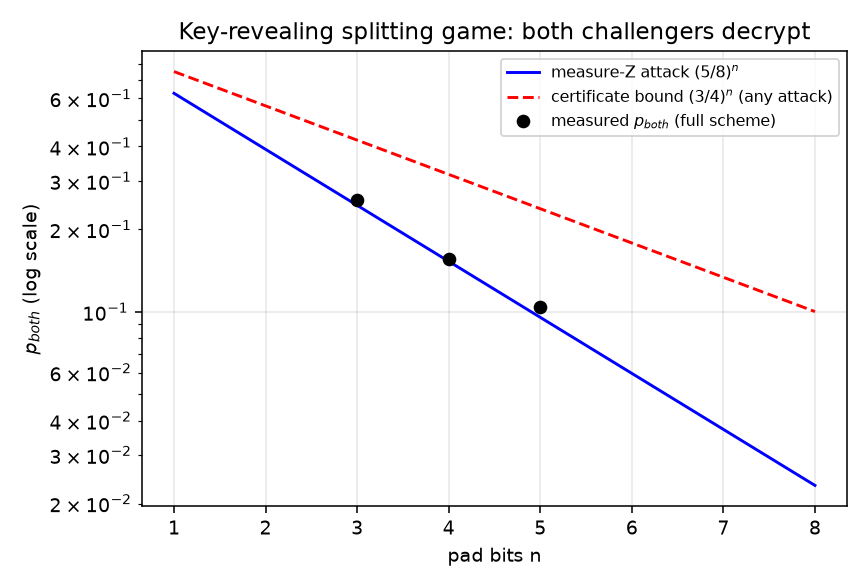
\includegraphics[width=0.7\textwidth]{../results/splitting_game.png}
\caption{$p_{\text{both}}$ versus $n$ (log scale): empirical scheme game, the
$(5/8)^n$ attack bound and the $(3/4)^n$ theorem ceiling.}
\label{fig:nbit}
\end{figure}

Scheme-level correctness and confidentiality numbers from
\texttt{scripts/run\_scheme.py} (\texttt{results/scheme.json}): 20/20 round
trips on the demo circuit (both pad instantiations); 60/60 correct evaluations
on random circuits, each also verified against an independent statevector
simulation of the physical circuit; linear scaling $n = 10$ to $10^4$ in
transcript mode with all outputs correct ($7.6\,\mathrm{ms}$ at $n=10^4$); and
a confidentiality check ($n = 6$, $4000$ samples) whose empirical distribution
of the transcript deviates from the ideal uniform-transcript distribution by at
most $4.9\times10^{-3}$, and from message to message by at most
$6.7\times10^{-3}$ --- statistical noise at that sample size.

\section{Scope, limitations and what is new}\label{sec:scope}

\textbf{Scope.}  Classical messages; one-time use of $(\theta, a)$ (the pad $a$
is a one-time pad, so key reuse would break confidentiality as in any OTP);
private-key setting; circuits over $\{\mathsf{NOT},\mathsf{AND}\}$ on $n$ wires
with distinct $\mathsf{AND}$ targets --- the Broadbent--Jeffery~\cite{bj15}
setting.  Security is against a single ciphertext held by one adversary who
splits it once, then both parties see $\theta$ (the key-revealing game of
\cite{bl20}); decoders are honest ($\theta$-basis measurement).  Allowing the
decoders arbitrary POVMs can only raise the value; numerically the SDP search
still returns $3/4$, but the analytic certificate here is stated for honest
decoding.

\textbf{What is not claimed.}  Compactness (the transcript is released),
multi-time security, quantum message encryption, and composition: this is a
first-principles construction with complete quantitative analysis in a narrow
setting, not a competitor to the general-message unconditional schemes of
\cite{as26,bbc26}.  Its point is the fusion: the uncloneable register \emph{is}
the pad, evaluation is exact at any depth precisely because the payload is
classical, and the uncloneability constant is not inherited from the literature
but recomputed here --- with a complete proof --- for the game the scheme
actually faces.

\appendix

\section{The dual certificate}\label{app:cert}

Order the $8$-dimensional space as input qubit $\otimes$ output pair in the
basis $(|0\rangle,|1\rangle) \otimes (|00\rangle,|01\rangle,|10\rangle,|11\rangle)$.
Evaluating $M = \tfrac14 \sum_u |u\rangle\langle u| \otimes |uu\rangle\langle uu|$
over $u \in \{|0\rangle,|1\rangle,|+\rangle,|-\rangle\}$ gives the exact rational
matrix
\[
  16\,M \;=\;
  \begin{pmatrix}
  5&0&0&1&0&1&1&0\\
  0&1&1&0&1&0&0&1\\
  0&1&1&0&1&0&0&1\\
  1&0&0&1&0&1&1&0\\
  0&1&1&0&1&0&0&1\\
  1&0&0&1&0&1&1&0\\
  1&0&0&1&0&1&1&0\\
  0&1&1&0&1&0&0&5
  \end{pmatrix},
\]
which is real symmetric.  Direct computation of the characteristic polynomial
(exact rational arithmetic; reproduced by \texttt{sympy} in the repository and
asserted numerically to $10^{-12}$ in \texttt{tests/test\_games.py}) gives
\[
  \chi_M(\lambda) \;=\; \lambda^4 \left(\lambda - \tfrac18\right)^2
  \left(\lambda - \tfrac38\right)^2 ,
\]
so $M \succeq 0$ and $\lambda_{\max}(M) = \tfrac38$.  With $Y = \tfrac38 I_2$ the
gap $S = Y \otimes I_4 - M$ has spectrum
$\{0, 0, \tfrac14, \tfrac14, \tfrac38, \tfrac38, \tfrac38, \tfrac38\} \subseteq
[0,\infty)$, i.e.\ $S \succeq 0$, and $\tr Y = \tfrac34$: exactly the
dual-feasible point used in Theorem~\ref{thm:value}.  The kernel of $S$ is
$\ker S = \operatorname{span}\{\operatorname{vec}(A_1),
\operatorname{vec}(A_2)\}$, where $A_1, A_2$ are the Kraus operators of
$\Lambda^\ast$ from Theorem~\ref{thm:value} (they are orthonormal
$\tfrac38$-eigenvectors of $M$, and the eigenspace is two-dimensional):
complementary slackness $\operatorname{tr}[J_{\Lambda^\ast} S] = 0$ holds
exactly, so primal and dual optima meet at $3/4$.  The repository asserts
$M \operatorname{vec}(A_k) = \tfrac38 \operatorname{vec}(A_k)$ numerically in
\texttt{tests/test\_games.py}.

\begin{thebibliography}{9}
\bibitem{bl20} A.\ Broadbent and J.\ Lord, \emph{Uncloneable Quantum Encryption
via Oracles}, in 5th Conference on the Theory of Quantum Computation,
Communication and Cryptography (TQC 2020), LIPIcs Vol.~158, Article~4,
pp.~4:1--4:22, 2020. doi:10.4230/LIPIcs.TQC.2020.4.
\bibitem{bj15} A.\ Broadbent and S.\ Jeffery, \emph{Quantum Homomorphisms for
Classical Circuits and Their Computational Power}, Quantum Info.\ Comput.\
15(7--8):635--672, 2015.
\bibitem{as26} P.\ Ananth and A.\ Sahai, \emph{Unconditional Unclonable
Encryption}, arXiv:2607.21551, 2026.
\bibitem{bbc26} A.\ Bhattacharyya, A.\ Broadbent and E.\ Culf, \emph{Statistically
secure uncloneable encryption of arbitrary messages}, arXiv:2607.28561, 2026.
\bibitem{bcr26} A.\ Broadbent, E.\ Culf and D.\ Rochette, \emph{Optimal
Untelegraphable Encryption and Implications for Uncloneable Encryption},
arXiv:2510.00903, 2025.
\bibitem{bw84} C.\ H.\ Bennett and D.\ J.\ Wiesner, \emph{Quantum cryptography
based on Bell's theorem}, Phys.\ Rev.\ Lett.\ 53:1921--1923, 1984.
\bibitem{watrous} J.\ Watrous, \emph{The Theory of Quantum Information},
Cambridge University Press, 2018.
\end{thebibliography}

\end{document}
